\documentclass[a4paper,aps,12pt,tightenlines]{revtex4-2}
\usepackage[a4paper,margin=0.75in]{geometry}
\usepackage[utf8]{inputenc}
\usepackage[T1]{fontenc}
\usepackage{microtype}
\usepackage[italian]{babel}
\makeatletter
\let\it@comma@def\active@comma
\makeatother
\usepackage{physics}
\usepackage{graphicx}
\usepackage{siunitx}
\usepackage[hidelinks]{hyperref}

\DeclareMathOperator{\Corr}{Corr}
\DeclareMathOperator{\Cov}{Cov}
\DeclareMathOperator{\E}{E}
\DeclareMathOperator{\Var}{Var}

\begin{document}
\count\footins = 1000
% \preprint{LMCS\_d0\_\today}
% \preprint{Electromagnetic-Waves-003/1}
\title{Misura delle righe di Balmer per H con metodi Monte Carlo}
%\author{A. Parodi}
\author{F. Polleri}
\email{s5025011@studenti.unige.it}
\author{M. Sotgia}
\email{s4942225@studenti.unige.it}
\affiliation{Dipartimento di Fisica, Università degli Studi di Genova, 16146 Genova, Italy}
\date{\today}
% \revised{\today}
\maketitle

\section{Introduzione}
Un prisma ottico può essere utilizzato, sfruttando il fenomeno della rifrazione, come spettrometro per eseguire misure precise della lunghezza d'onda dato un fascio monocromatico incidente, in grado anche di separare le componenti di un fascio non monocromatico. 

Si sa che infatti la differenza $\delta_i$ tra l'angolo in ingresso $\theta_0$ e l'angolo in uscita $\theta_i$ risulta essere legato al valore dell'indice di rifrazione del materiale, \begin{equation}\delta_i = \theta_0 - \alpha+\arcsin\left(n\sin\left(\alpha - \arcsin\left(\frac{\sin\theta_0}{n}\right)\right)\right),\end{equation} con $n$ indice di rifrazione e $\alpha$ apertura angolare del prisma. 

Si osserva che $\delta_i$ ha un minimo in corrispondenza del quale la misura è più stabile e la relazione precedente si semplifica come \begin{equation} n\sin\frac{\alpha}{2} = \sin\frac{\delta_m + \alpha}{2} = \sin\theta_{0_m}.\end{equation}

Da quest'ultima relazione possiamo ottenere una forma per l'indice \begin{equation} n(\theta, \theta_0) = \frac{\sin\frac{\theta-\theta_0 + \alpha}{2}}{\sin\frac{\alpha}{2}}.\label{eq:nthth0}\end{equation}

Possiamo anche però ricavare la relazione che lega l'indice di rifrazione $n$ al valore di $\delta_m$, e poichè $n=n(\lambda)$, secondo la relazione di Cauchy \begin{equation} n(\lambda) = A + \frac{B}{\lambda^2},\end{equation} appropriata ad un ordine $\mathcal O (1/\lambda^2)$, con $A$ e $B$ coefficienti propri del materiale in questione, allora possiamo concludere che esistono relazioni che legano $\lambda$ con il valore di $\delta_i$. 

\subsection{Angoli di Balmer}

Data la lunghezza d'onda, in cui si osservano rispetto ad un elemento le bande di assorbimento o di emissione, viene definita da Balmer una relazione che permette di quantificare la posizione di queste bande \begin{equation} \frac{1}{\lambda} = R_H \qty(T(n) - T(m)) \end{equation} che nel caso dell'idrogeno assume una forma particolarmente comoda, dove $T(n) = 1/n^2$. Otteniamo quindi una equazione del tipo \begin{equation} \frac{1}{\lambda} = R_H \qty(\frac{1}{n^2} - \frac{1}{m^2}). \label{eq:ryd}\end{equation} Queste lunghezze d'onda corrispondono implicitamente ad alcuni angoli determinati dallo strumento appena caratterizzato. 

\section{Misura della costante di Rydberg}

Un utilizzo che possiamo fare delle relazioni fino ad ora trovate, e dello strumento che abbiamo descritto, è quello di sfruttarlo per ottenere una stima del parametro $R_H$, detto costante di Rydberg, dalla relazione degli angoli di Balmer. Sono noti gli angoli $\theta_m$ ai quali si trovano le bande di emissione dell'idrogeno, per $m = 3, 4, 5, 6$ e $n=2$, e si conoscono i parametri $A$, $B$ con le loro distribuzioni e il coefficiente di correlazione che esiste tra i due, $\rho_{AB}$.

Possiamo allora determinare per ogni $\theta_m$ il valore $\lambda_m$ come \begin{equation} \frac{1}{\lambda_m} =  \sqrt{\frac{n(\theta, \theta_0) - A}{B}}, \label{eq:7}\end{equation} dove $n(\theta, \theta_0)$ è fornito dalla Eq. (\ref{eq:nthth0}). 
Possiamo quindi chiaramente trovare una relazione tra i dati forniti e il valore di $R_H$. 
Obiettivo primario è quindi calcolare il valore delle lugnhezze d'onda a partire dai dati conosciuti. Conosciamo la forma effettiva di $\frac{1}{\lambda} = \frac{1}{\lambda}(\theta, \theta_0, A, B, \alpha)$, dove, a parte $\alpha$, i parametri presentano deviazione standard non trascurabile, comportando una correlazione tra i valori $\lambda_m$ al variare di $m$. Inoltre, prima ancora di incontrare il problema legato alla correlazione tra le diverse lunghezze d'onda, dobbiamo capire come procedere per poterle ottenere, con anche una loro deviazione standard. Dalle relazioni (\ref{eq:7}) e (\ref{eq:ryd}) osserviamo che la quantità che in realtà è utile ottenere è il fattore $1/\lambda$, comune alle due equazioni. 

Possiamo osservare che la dipendenza della lunghezza d'onda dai suoi parametri è molto probabilmente non lineare (si può vedere solo dalla radice quadrata che si ha per ottenere il valore di $1/\lambda$), senza considerare che $A$ e $B$ sono tra loro legati da un coefficente di correlazione $\rho_{A,B}$. L'unico modo per ottenere il valore di $1/\lambda$ sarà quindi procedendo con metodi Monte Carlo (da qui in avanti MC). I parametri che presentano errore associato, e che non sono correlati tra loro e con le altre variabili ($\theta_m$, $\theta_0$), sono ipotizzati essere distribuiti secondo una Gaussiana, centrata nel calor medio $\mu_i$ e deviazione standard $\sigma_i$, con $i=\theta_m$, $\theta_0$. Il parametro $\alpha$ è considerato privo di errore. Supponendo di poter considerare $A$, $B$ come distribuzioni Gaussiane di valor medio $\mu_A$, $\mu_B$ e deviazione standard $\sigma_A$, $\sigma_B$ resta da capire come possiamo generare valori di $A$, $B$ che presentano invece coefficente di correlazione $\rho_{A,B} = \num{-0.872}$. Analizziamo in seguito il problema.

\subsection{Generazione di variabili correlate}
\emph{Il risultato che si ottiene è frutto di una ricerca e non tutto farina del nostro sacco, i crediti vanno a \cite{anthonyAnswerHowDoes2015, sobolevAnswerHowDoes2015, kaiserSamplePopulationScore1962}, anche se siamo riusciti a rieseguire i calcoli e trovare la soluzione proposta. }

\begin{figure*}
\centering
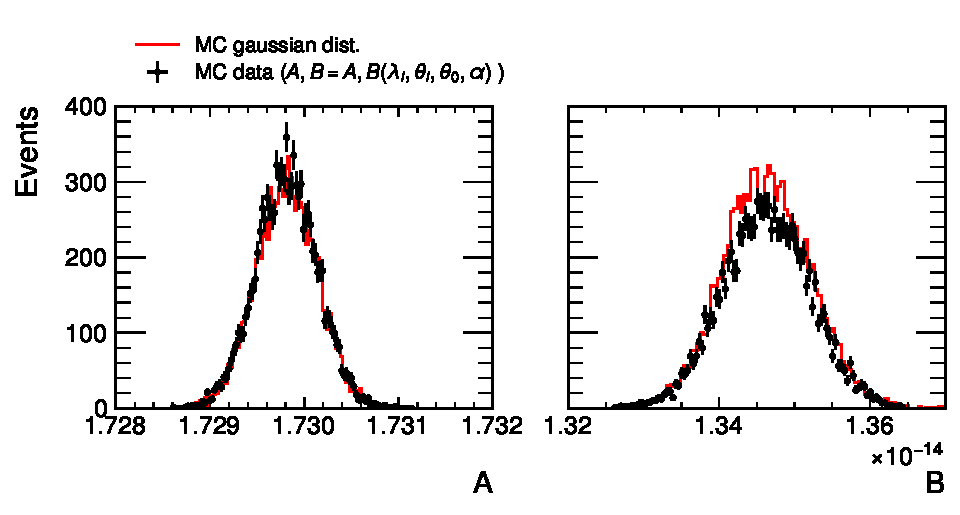
\includegraphics{../figures_and_tests/gaus_compAB.pdf}
\caption{Abbiamo generato $A$, $B$ prima utilizzando le formule, quindi a partire da $\lambda_i, \theta_i, \theta_0, \alpha$, poi utilizzando media e deviazione standard abbiamo ricostruito $A$ e $B$ come distribuzioni gaussiane, riportate in rosso.}
\end{figure*}

Sapendo che le distribuzioni di $A$, $B$ corrispondono a distribuzioni Gaussiane (fig. \ref{fig:A_B_gaus}), possiamo ipotizzare che siano legate tra loro imponendo che \begin{equation} \left\{ 
    \begin{aligned}
        & A = x_1 X _1 + x_2 X_2\\
        & B = X_1
    \end{aligned}
\right.\label{eq:8}
\end{equation}
con $x_1, x_2$ ignote e $X_1, X_2$ distribuzioni che consideriamo essere gaussiane. Sappiamo inoltre che \begin{equation} \Corr[A,B] = \rho = \frac{\Cov[A,B]}{\sqrt{\Var[A]\Var[B]}} =  \frac{x_1\Cov[X_1, X_1]}{\sqrt{x_1^2\Var[X_1] + x_2^2\Var[X_2]}} = \frac{x_1\sigma_1^2}{\sqrt{x_1\sigma_1^2+x_2\sigma_2^2}},\end{equation} oltre a sapere che \begin{equation} \rho = x_1\frac{\sigma_B}{\sigma_A} \implies x_1 = \rho\frac{\sigma_A}{\sigma_B}, \end{equation} dove abbiamo considerato che $\sigma_B = \sigma_1$ e $\mu_B = \mu_1$. 

Dalle relazioni in \eqref{eq:8} abbiamo ottenuto il sistema \begin{equation}\left\{
    \begin{aligned}
        \mu_A &= x_1 \mu_1 + x_2 \mu_2\\
        \mu_B &= \mu_1\\
        \sigma_A^2 &= x_1^2\sigma_1^2 + x_2^2\sigma_2^2\\
        \sigma_B^2 &= \sigma_1^2,
    \end{aligned}
\right.
\end{equation}
da cui abbiamo che, con le dovute sostituzioni, \begin{equation}\left\{
    \begin{aligned} 
    x_1 &= \rho \frac{\sigma_A}{\sigma_B}\\
    x_2 &= \sigma_A \sqrt{1-\rho^2}\\
    \mu_1 &= \mu_B\\
    \sigma_1 &= \sigma_B\\
    \mu_2 & = \left(\frac{\mu_A}{\sigma_A} - \rho\frac{\mu_B}{\sigma_B}\right)\frac{1}{\sqrt{1-\rho^2}}\\
    \sigma_2 &= 1
    \end{aligned}
\right.
\end{equation}

Abbiamo quindi la possibilità di generare in modo coerente con quanto atteso il valore di $A$ e il valore di $B$, generando quindi $B$ secondo una distribuzione Gaussiana $(\mu_B, \sigma_B)$ e ottenendo invece $A$ come $A=\rho \frac{\sigma_A}{\sigma_B}\cdot B + \sigma_A \sqrt{1-\rho^2} \cdot X_2$, con $X_2$ generata come una Gaussiana \begin{equation}\left\{\begin{aligned}\mu_2 &= \left(\frac{\mu_A}{\sigma_A} - \rho\frac{\mu_B}{\sigma_B}\right)\frac{1}{\sqrt{1-\rho^2}}\\\sigma_2 &= 1\end{aligned}\right.\end{equation}.

\subsection{Valori di $R_H$ dagli angoli di Balmer}

Con metodi MC possiamo ora trovare i valori di $1/\lambda$, e poi conoscendo la \eqref{eq:ryd} potremmo realizzare un fit lineare per trovare il parametro $R_H$. Se considerassimo un fit minimizzando il valore del $\chi^2$ in maniera standard potremmo non coniderare i coefficenti di correlazione che esistono dovuti al modo in cui stiamo calcolando i valori di $1/\lambda_m$, che dipendono tutti dagli stessi valori (con errore associato non trascurabile) di $A$, $B$ e $\theta_0$. 

Però possiamo caloclare per ogni coppia $(m, \lambda_m)$, o meglio $(m, 1/\lambda_m)$, un valore di $R_{H,m}$, considerando quindi una soluzione del tipo \begin{equation} 
    R_{H,m} = \frac{n^2m^2}{m^2-n^2}\sqrt{\frac{1}{B} \qty(\frac{\sin\frac{\theta_m-\theta_0 + \alpha}{2}}{\sin\frac{\alpha}{2}}-A)},
\end{equation} dove $\alpha$ è considerato privo di errore, $\theta_m, \theta_0$ sono considerati con errore, $n=2$, $m=3,4,5,6$ sono privi di errori, e $A$, $B$ sono generati come definito prima. Considerata questa relazione possiamo generare $N_\text{exp}$ esperimenti per ogni coppia $(m, \theta_m)$, per ognuno dei quali otteniamo il valore di $R_{H,m}$ per ogni valore di $m$, e possiamo così avere quattro distribuzioni per $R_H$ corrispondenti ai rispettivi valori di $m$ (come in fig. \ref{fig:rydberg}). 

\begin{figure}
\centering
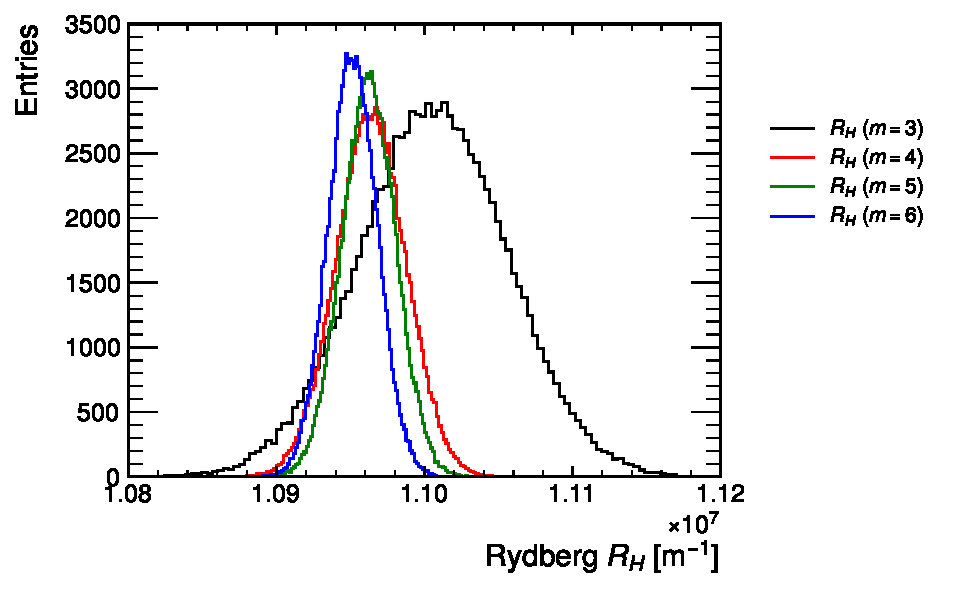
\includegraphics[]{../figures_and_tests/rydberg.pdf}
\caption{possiamo generare $N_\text{exp}$ esperimenti per ogni coppia $(m, \theta_m)$, per ognuno dei quali otteniamo il valore di $R_{H,m}$ per ogni valore di $m$, e possiamo così avere quattro distribuzioni per $R_H$ corrispondenti ai rispettivi valori di $m$. \label{fig:rydberg}}
\end{figure}

\bibliography{corr_matrix_formula}

\end{document}